\section{Bất phương trình bậc nhất hai ẩn}
\setcounter{dang}{0}
\subsection{Tóm tắt lý thuyết}
\subsubsection{Bất phương trình bậc nhất hai ẩn}
Bất phương trình bậc nhất hai ẩn $x$, $y$ có dạng tổng quát là 
\begin{center}
\fbox{$ax+by\le c \text{ (hoặc } ax+by<c; ax+by\ge c; ax+by>c),$}
\end{center}
trong đó $a$, $b$, $c$ là những số thực, $a$ và $b$ không đồng thời bằng $0$, $x$ và $y$ là các ẩn số.

\subsubsection{Biểu diễn tập nghiệm của bất phương trình bậc nhất hai ẩn}
Cũng như bất phương trình bậc nhất một ẩn, các bất phương trình bậc nhất hai ẩn có vô số nghiệm và để mô tả tập nghiệm của chúng, ta sử dụng phương pháp biểu diễn hình học.\\ 
Trong mặt phẳng tọa độ $Oxy$, tập hợp các điểm có tọa độ là nghiệm của bất phương trình được gọi là \textbf{miền nghiệm} của nó.\\
Quy tắc thực hành biểu diễn miền nghiệm của bất phương trình $ax+by \le c$ như sau (tương tự cho bất phương trình $ax+by\ge c$)
\begin{itemize}
	\item{\bf Bước 1:} Trên mặt phẳng tọa độ $Oxy$, vẽ đường thẳng $\Delta \colon ax+by=c$.
	\item{\bf Bước 2:} Lấy một điểm $M_0\left(x_0;y_0\right)$ không thuộc $\Delta$ (ta thường lấy gốc tọa độ $O$).
	\item{\bf Bước 3:} Tính $ax_0+by_0$ và so sánh $ax_0+by_0$ với $c$.
	\item{\bf Bước 4:} Kết luận,
	\begin{itemize}
		\item Nếu $ax_0+by_0<c$ thì nửa mặt phẳng bờ $\Delta$ chứa $M_0$ là miền nghiệm của $ax_0+by_0\leq c$.
		\item Nếu $ax_0+by_0>c$ thì nửa mặt phẳng bờ $\Delta$ không chứa $M_0$ là miền nghiệm của $ax_0+by_0\le c$.
	\end{itemize}
\end{itemize}

\begin{note}
	Miền nghiệm của bất phương trình $ax_0+by_0\leq c$ bỏ đi đường thẳng $ax+by=c$ là miền nghiệm của bất phương trình $ax_0+by_0<c$.
\end{note}
\subsection{Các dạng toán}
\begin{dang}{Bất phương trình bậc nhất hai ẩn và bài toán liên quan}
\end{dang}
\viduminhhoa
\begin{vd}%[Dự án Tex hóa đề thi lớp 10-11-Nhóm Word-T-Begin]%[Lê Vũ Hải-Phản biện: Trần Quốc Tráng]%[0D4Y4-1]%
	Cho bất phương trình: $2x-y<0$ . Trong các cặp số $(-1;2)$, $\left(2;0\right)$, $(0;1)$, $\left(3;-2\right)$, $(-1;-2)$, cặp nào là nghiệm của bất phương trình, cặp nào không phải là nghiệm của bất phương trình?
	\loigiai{
		Bằng cách thử trực tiếp, các cặp $(-1;2)$, $(0;1)$ là nghiệm, các cặp còn lại không phải là nghiệm của bất phương trình.
	}
\end{vd}
\begin{vd}%[Dự án Chuyển tex 10-11, Cao Thành Thái]%[0D4B4-1]
	Biểu diễn hình học tập nghiệm của bất phương trình $2x+y\le 3$.
	\loigiai
	{
		\immini{
			Vẽ đường thẳng $\Delta\colon 2x+y=3$.\\
			Lấy gốc tọa độ $O(0;0)$, ta thấy $O\notin \Delta $ và có $2 \cdot 0+0<3$ nên nửa mặt phẳng bờ $\Delta$ chứa gốc tọa độ $O$ là miền nghiệm của bất phương trình đã cho (miền không bị tô đậm trong hình vẽ).
		}
		{
			\begin{tikzpicture}[line join=round, line cap=round, >=stealth,font=\footnotesize, scale=0.8]
				\draw[->](-2,0)--(3,0) node[below right] {$x$};
				\draw[->](0,-1)--(0,4) node[right] {$y$};
				\clip (-2,-1) rectangle (3,4);
				\node (0,0) [below left]{$ O $};
				\foreach \x in {-1,...,2}
				\draw[shift={(\x,0)},color=black] (0pt,2pt) -- (0pt,-2pt);
				\foreach \y in {1,...,3}
				\draw[shift={(0,\y)},color=black] (2pt,0pt) -- (-2pt,0pt);
				\draw[samples=100,smooth,domain=-2:3] plot(\x,{-2*(\x)+3});
				\draw [pattern=north west lines] (-1,5)--(3,5)--(3,-1) -- (2,-1)--cycle;
				\draw[fill=black] (0,3) circle(1pt) node[left]{$3$};
				\draw[fill=black] (1.5,0)circle(1pt) node[below left]{\tiny $\dfrac{3}{2}$};
			\end{tikzpicture}
		}
	}
\end{vd}
\begin{vd}%[Mai Hà Lan]%[0D4B4-1]
	\begin{enumerate}
		\item Biểu diễn hình học tập nghiệm của bất phương trình $-2x + 3y > 0$.
		\item Cho hai điểm $A(2;1)$ và $B(3; 3)$, hỏi hai điểm này cùng phía hay khác phía đối với bờ $(d)$.
	\end{enumerate}
	\loigiai{
		\immini{
			\begin{enumerate}
				\item Vẽ đường thẳng $d: -2x + 3y = 0$.\\
				Thay tọa độ điểm $M(1;0)$ vào vế trái phương trình đường thẳng $(d)$, ta được: $-2 < 0$.\\
				Vậy miền nghiệm của bất phương trình là nửa mặt phẳng không chứa điểm $M$. (Trên hình là nửa mặt phẳng không bị gạch bỏ).
				\item Thế tọa độ điểm $A$ vào vế trái của phương trình đường thẳng $(d)$ ta được $-2 \cdot 2 + 3 \cdot 1 = -1 < 0$.\hfill $(1)$\\
				Thế tọa độ điểm $B$ vào vế trái của phương trình đường thẳng $(d)$ ta được $-2 \cdot 3 + 3 \cdot 3 = 3 > 0$. \hfill $(2)$ \\
				Từ $(1)$ và $(2)$ suy ra hai điểm nằm ở hai phía đối với bời $(d)$.
			\end{enumerate}
		}{
			\begin{tikzpicture}
				%---------------------- Vẽ hệ trục tọa độ
				\draw[->] (-2.25,0)--(4.25,0) node[below right] {$x$};
				\draw[->] (0,-0.755)--(0,2.25) node[right] {$y$};
				\node (0,0) [below right]{$ O $};
				%----------------------- Vẽ đoạn chắn trên trục
				\foreach \x in {-2,-1,1,2,3,4}
				\draw[shift={(\x,0)},color=black] (0pt,2pt) -- (0pt,-2pt);
				%\node at (3.8,0.5) {$4$};
				\foreach \y in {1,2}
				\draw[shift={(0,\y)},color=black] (2pt,0pt) -- (-2pt,0pt);
				%\node at (-0.5,-1.8) {$-2$};
				
				%--------------------- Vẽ hàm
				\draw [thick, domain=-1:3, samples=100] plot (\x, {(2/3) * \x});
				\node at (2,1.75) {$(d)$};
				
				%---------------------- Điểm M
				\fill (1,0) circle (2pt) node[below right]{$M(1;0)$};
				
				%----------------------Vẽ miền nghiệm
				\tkzDefPoints{-1/-.66/A, 4/-.66/B, 4/2/C, 3/2/D}
				\tkzDrawPolygon[ pattern=north east lines,opacity=.3](A,B,C,D)
			\end{tikzpicture}
	}}
\end{vd}
\begin{vd}%[Mai Hà Lan]%[0D4G4-1]
	\begin{enumerate}
		\item Biểu diễn hình học tập nghiệm của bất phương trình $x + y -3 < 0$.
		\item Tìm điều kiện của $m$ và $n$ để mọi điểm thuộc đường thẳng $(d')$: $ (m^2-2)x - y + m + n= 0 $ đều là nghiệm của bất phương trình trên.
	\end{enumerate}
	\loigiai{
		\immini{
			\begin{itemize}
				\item[a)] Vẽ đường thẳng $d: x + y = 3 $.\\
				Thay tọa độ điểm $O(0;0)$ vào vế trái phương trình đường thẳng $(d)$, ta được: $0< 3$.\\
				Vậy miền nghiệm của bất phương trình là nửa mặt phẳng chứa điểm $O$. (Trên hình là nửa mặt phẳng không bị gạch bỏ).
				\item[b)] Để mọi điểm thuộc đường thẳng  $(d')$ đều là nghiệm của bất phương trình thì điều kiện cần là $(d')$ phải song song với $(d)$. Ta có $d:  y = -x + 3$ và $d': y = (m^2-2)x +  m + n$. Để $(d)$ song song $(d')$ thì $\heva{& m^2 - 2 = -1 \\& m + n \ne 3} \Leftrightarrow \hoac{&\heva{&m=1\\&n\ne 2}\\&\heva{&m=-1\\&n\ne 4}}$\\
				Với $\heva{&m=1\\&n\ne 2}$ thì ta được $d': y = - x + n + 1$. Để thỏa yêu cầu bài toán thì điều kiện đủ là đường thẳng $(d')$ là đồ thị của đường thẳng $(d)$ khi $(d)$ tịnh tiến xuống dưới theo trục $Oy$. Tức $n + 1 < 3 \Leftrightarrow n < 2$.
			\end{itemize}
		}{
			\begin{tikzpicture}[scale=.8]
				%---------------------- Vẽ hệ trục tọa độ
				\draw[->] (-2.25,0)--(4.25,0) node[below right] {$x$};
				\draw[->] (0,-1.25)--(0,4.25) node[right] {$y$};
				\node (0,0) [below left]{$ O $};
				%----------------------- Vẽ đoạn chắn trên trục
				\foreach \x in {-2,-1,1,2,3,4}
				\draw[shift={(\x,0)},color=black] (0pt,2pt) -- (0pt,-2pt);
				\node at (2.75,-0.4) {$3$};
				\foreach \y in {-1,1,2,3,4}
				\draw[shift={(0,\y)},color=black] (2pt,0pt) -- (-2pt,0pt);
				\node at (-0.35,2.75) {$3$};
				
				%--------------------- Vẽ hàm
				\draw [thick, domain=-1:4, samples=100] plot (\x, {3-\x});
				\node at (1.2,1.2) {$(d)$};
				
				%----------------------Vẽ miền nghiệm
				\tkzDefPoints{-1/4/A, 4/4/B, 4/-1/C}
				\tkzDrawPolygon[pattern=north east lines,opacity=.3](A,B,C)
			\end{tikzpicture}
	}}
\end{vd}
\baitaptl
\begin{bt}%[Dự án Chuyển tex 10-11, Cao Thành Thái]%[0D4B4-1]%
	Biểu diễn hình học tập nghiệm của bất phương trình $2x+y\le 3$.
	\loigiai
	{
		\immini{
			Vẽ đường thẳng $\Delta\colon 2x+y=3$.\\
			Lấy gốc tọa độ $O(0;0)$, ta thấy $O\notin \Delta $ và có $2 \cdot 0+0<3$ nên nửa mặt phẳng bờ $\Delta$ chứa gốc tọa độ $O$ là miền nghiệm của bất phương trình đã cho (miền không bị tô đậm trong hình vẽ).
		}
		{
			\begin{tikzpicture}[line join=round, line cap=round, >=stealth,font=\footnotesize, scale=0.8]
				\draw[->](-2,0)--(3,0) node[below right] {$x$};
				\draw[->](0,-1)--(0,4) node[right] {$y$};
				\clip (-2,-1) rectangle (3,4);
				\node (0,0) [below left]{$ O $};
				\foreach \x in {-1,...,2}
				\draw[shift={(\x,0)},color=black] (0pt,2pt) -- (0pt,-2pt);
				\foreach \y in {1,...,3}
				\draw[shift={(0,\y)},color=black] (2pt,0pt) -- (-2pt,0pt);
				\draw[samples=100,smooth,domain=-2:3] plot(\x,{-2*(\x)+3});
				\draw [pattern=north west lines] (-1,5)--(3,5)--(3,-1) -- (2,-1)--cycle;
				\draw[fill=black] (0,3) circle(1pt) node[left]{$3$};
				\draw[fill=black] (1.5,0)circle(1pt) node[below left]{\tiny $\dfrac{3}{2}$};
			\end{tikzpicture}
		}
	}
\end{bt}
\begin{bt}%[0D4B4-1]%
	Biểu diễn hình học tập nghiệm của bất phương trình bậc nhất hai ẩn $2x - 4y < 8$.
	\loigiai{
		\immini{
			Vẽ đường thẳng $d: 2x - 4y =8$.\\
			Thay tọa độ điểm $O(0;0)$ vào vế trái phương trình đường thẳng $(d)$, ta được: $0 < 8$.\\
			Vậy miền nghiệm của bất phương trình là nửa mặt phẳng chứa điểm $O$. (Trên hình là nửa mặt phẳng không bị gạch bỏ).
		}{
			\begin{tikzpicture}[scale=.7]
				%----------------- Vẽ hệ trục tọa độ
				\draw[->] (-2.25,0)--(8.25,0) node[below right] {$x$};
				\draw[->] (0,-3.25)--(0,1.25) node[right] {$y$};
				\node (0,0) [below left] {$ O $};
				%----------------- Vẽ đoạn chắn trên trục
				\foreach \x in {-2,-1,1,2,3,4,5,6,7,8}
				\draw[shift={(\x,0)},color=black] (0pt,2pt) -- (0pt,-2pt);
				\node at (3.8,0.5) {$4$};
				\foreach \y in {-3,-2,-1,1}
				\draw[shift={(0,\y)},color=black] (2pt,0pt) -- (-2pt,0pt);
				\node at (-0.5,-1.8) {$-2$};
				
				%------------- Vẽ hàm
				\draw [thick, domain=-2:6, samples=100] plot (\x, {(1/2)*\x - 2});
				\node at (4.5,.75) {$(d)$};
				
				%---------------- Vẽ miền nghiệm
				\tkzDefPoints{6/1/A, -2/-3/B, 8/-3/C, 8/1/D}
				\tkzDrawPolygon[ pattern=north east lines,opacity=.3](A,B,C,D)
			\end{tikzpicture}
	}}
\end{bt}
\begin{bt}%[Mai Hà Lan]%[0D4B4]
	Biểu diễn hình học tập nghiệm của bất phương trình bậc nhất hai ẩn $3x - y \le 0$.
	\loigiai{
		\immini{
			Vẽ đường thẳng $d: 3x - y = 0 $.\\
			Thay tọa độ điểm $M(0;2)$ vào vế trái phương trình đường thẳng $(d)$, ta được: $-2 < 0$.\\
			Vậy miền nghiệm của bất phương trình là nửa mặt phẳng không chứa điểm $M$, kể cả bờ $(d)$. (Trên hình là nửa mặt phẳng không bị gạch bỏ).
		}{
			\begin{tikzpicture}
				%---------------------- Vẽ hệ trục tọa độ
				\draw[->] (-2.25,0)--(2.25,0) node[below right] {$x$};
				\draw[->] (0,-1.25)--(0,3.25) node[right] {$y$};
				\node (0,0) [above right]{$ O $};
				%----------------------- Vẽ đoạn chắn trên trục
				\foreach \x in {-2,-1,1}
				\draw[shift={(\x,0)},color=black] (0pt,2pt) -- (0pt,-2pt);
				%\node at (3.8,0.5) {$4$};
				\foreach \y in {-1,1,2,3}
				\draw[shift={(0,\y)},color=black] (2pt,0pt) -- (-2pt,0pt);
				%\node at (-0.5,-1.8) {$-2$};
				
				%--------------------- Vẽ hàm
				\draw [thick, domain=-.33:1, samples=100] plot (\x, {3*\x});
				\node at (.5,2.5) {$(d)$};
				
				%---------------------- Điểm M
				\fill (0,2) circle (2pt) node[left]{$M(0;2)$};
				
				%----------------------Vẽ miền nghiệm
				\tkzDefPoints{-.33/-.99/A, 2/-1/B, 2/3/C, 1/3/D}
				\tkzDrawPolygon[ pattern=north east lines,opacity=.3](A,B,C,D)
			\end{tikzpicture}
	}}
\end{bt}
\begin{bt}%[Mai Hà Lan]%[0D4K4]
	a) Biểu diễn hình học tập nghiệm của bất phương trình bậc nhất hai ẩn $\dfrac{x}{3} + \dfrac{y}{6} < 1$.\\
	b) Tìm điểm $A$ thuộc miền nghiệm của bất phương trình trên. Biết rằng điểm $A$ là giao điểm của parabol $(P)$ có dạng $y = x^2 - 5x +4$ và trục hoành. 
	\loigiai{
		\immini{
			\begin{itemize}
				\item[a)] $\dfrac{x}{3} + \dfrac{y}{6} < 1 \Leftrightarrow 2x + y  <6$\\
				Vẽ đường thẳng $d: 2x + y = 6$.\\
				Thay tọa độ điểm $O(0;0)$ vào vế trái phương trình đường thẳng $(d)$, ta được: $0 < 6$.\\
				Vậy miền nghiệm của bất phương trình là nửa mặt phẳng chứa điểm $O$. (Trên hình là nửa mặt phẳng không bị gạch bỏ).
				\item[b)] Điểm $A$ nằm trên parabol $(P)$ có dạng $y = x^2 - 5x +4$ và trục hoành nên hoành độ của $A$ là nghiệm của phương trình $x^2 - 5x + 4 = 0 \Leftrightarrow \hoac{& x = 1\\ & x = 4.}$ \\
				Suy ra ta được hai điểm $(1;0)$ và $(4;0)$. Lần lượt thế tọa độ từng điểm vào vế trái của phương trình đường thẳng $(d)$, do $A$ thuộc miền nghiệm của bất phương trình đã cho nên ta được $A$ có tọa độ là $(1;0)$.
			\end{itemize}
		}{
			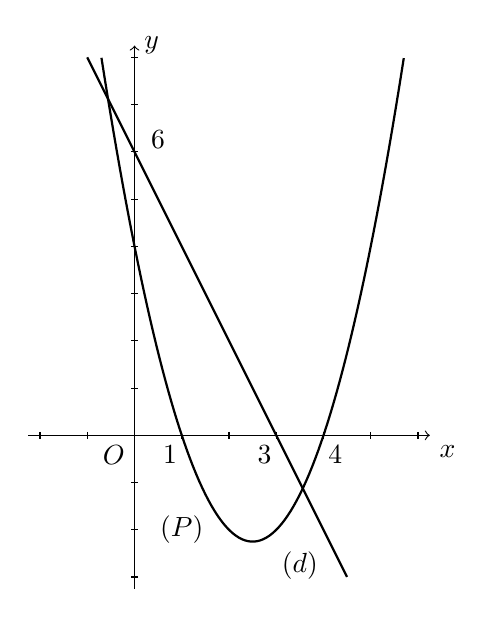
\begin{tikzpicture}[scale=.6]
				%---------------------- Vẽ hệ trục tọa độ
				\draw[->] (-2.25,0)--(6.25,0) node[below right] {$x$};
				\draw[->] (0,-3.25)--(0,8.25) node[right] {$y$};
				\node (0,0) [below left]{$ O $};
				%----------------------- Vẽ đoạn chắn trên trục
				\foreach \x in {-2,-1,1,2,3,4,5,6}
				\draw[shift={(\x,0)},color=black] (0pt,2pt) -- (0pt,-2pt);
				\node at (2.75,-0.4) {$3$};
				\node at (.75,-0.4) {$1$};
				\node at (4.25,-0.4) {$4$};
				\foreach \y in {-3,-2,-1,1,2,3,4,5,6,7,8}
				\draw[shift={(0,\y)},color=black] (2pt,0pt) -- (-2pt,0pt);
				\node at (0.5,6.25) {$6$};
				
				%--------------------- Vẽ hàm
				\draw [thick, domain=-1:4.5, samples=100] plot (\x, {-2*\x + 6});
				\node at (3.5,-2.75) {$(d)$};
				
				%---------------------- Vẽ (P)
				\draw [thick, domain=-.7:5.7, samples=100] plot (\x, {(\x)^2 - 5*\x + 4});
				\node at (1,-2) {$(P)$};
				
				%----------------------Vẽ miền nghiệm
				\tkzDefPoints{-1/8/A, 6/8/B, 6/-3/C, 4.5/-3/D}
				\tkzDrawPolygon[pattern=north east lines,opacity=.3](A,B,C,D)
			\end{tikzpicture}
	}}
\end{bt}
\begin{bt}%[Lê Xuân Dũng]%[0D4B4]%[0D4K4]
	Cho bất phương trình $2x+y-1 \le 0$.
	
	a) Biểu diễn miền nghiệm của bất phương trình đã cho trong mặt phẳng tọa độ $Oxy.$
	
	b) Tìm tất cả giá trị  tham số $m$ để điểm $M(m,1)$ nằm trong miền nghiệm của bất phương trình đã và biểu diễn tập
	hợp $M$ tìm được trong cùng hệ trục tọa độ $Oxy$ ở câu a).
	\loigiai{
		\immini{a) Đường thẳng $(d){:} \, 2x+y-1=0$ có đồ thị như hình vẽ bên.
			Ta có $2.0+0-1 <0.$ Do đó, miền nghiệm là đường thẳng $(d)$ và miền không gạch chéo như hình vẽ bên (Miền chứa gốc tọa độ).
			
			b) Để $M$ là một nghiệm thì $2m+1-1 \le 0\Leftrightarrow m\le 0.$ 
			Vì $M$ nằm trên đường thẳng $(\Delta): y = 1.$ Do đó, tập hợp tất cả điểm $M$
			là nghiệm của bất phương trình trình đã cho là tia $At$ như hình vẽ.
		}{\begin{tikzpicture}[scale=0.7,thick,>=stealth']
				\draw[->] (-1.3,0) -- (3.3,0)node[above]{$x$};
				\foreach \x in {}
				\draw[shift={(\x,0)},color=black] (0pt,2pt) -- (0pt,-2pt) node[below] {\footnotesize $\x$};
				\draw[->,color=black] (0,-2) -- (0,3.3)node[right]{$y$};
				\foreach \y in {}
				\draw[shift={(0,\y)},color=black] (2pt,0pt) -- (-2pt,0pt) node[left] {\footnotesize $\y$};
				\node[below left] at (0,0) {$O$};
				\node[below left] at (0,1) {$A$};
				\node[below] at (1,-1.3) {$d$};
				\node[above right] at (0,1) {$1$};
				\node[below] at (0.5,0) {$\frac{1}{2}$};
				\clip(-1.3,-2) rectangle (3,3);
				\node[below] at (-1.2,1) {$t$};
				%	\fill[pattern=north east lines] (-1,2.66667) -- (-1,4) -- (4,4) -- (4,-0.6667) -- (3,0) -- cycle;
				%\draw[line width=1.2pt,smooth,samples=100,domain=-1:4] plot(\x,{2-0.666667*(\x)});
				\fill[pattern=north east lines,pattern color=blue!30] (-1,3)--(0,1)--(0.5,0)--(1.5,-2)--(3,-2)--(3,0)--(3,3)-- cycle;
				\draw[line width=1.2pt,smooth,samples=100,domain=-3:3] plot(\x,{1-2*(\x)});
				\draw[line width=1.2pt][-] (0,1)--(-1.3,1);
		\end{tikzpicture}}
	}
\end{bt}

\begin{bt}%[Lê Xuân Dũng]%[0D4B4]%[0D4K4]
	Cho bất phương trình $x-2y+4m > 0.$
	
	a) Tùy theo giá trị tham số $m,$ hãy biểu diễn tập nghiệm của bất phương trình đã cho
	trong hệ trục tọa độ $Oxy.$
	
	b) Gọi $A,B$ lần lượt  là giao của đường thẳng $x-2y+4m=0$ với trục hoành và trục tung. 
	Tìm tất cả các giá trị của tham số $m$ để tập nghiệm của bất phương trình đã cho chứa điểm $C(2;1)$ 
	sao cho diện tích tam giác $ABC$ bằng $4.$
	\loigiai{
		\immini{a) Xét đường thẳng  $(d_m){:} \, x-2y+4m=0$ có đồ thị như hình vẽ bên.
			Ta có $0-2.0+4m = 4m.$ Do đó, với mọi $m \ne 0$ miền nghiệm luôn chứa gốc tọa độ.
			Nếu $m=0$ thì miền nghiệm chứa điểm $(1;0).$ Vậy với mọi $m$ miền nghiệm
			là miền không gạch chéo như hình vẽ bên.
			
			b) Để $C$ là một nghiệm của bất phương trình đã cho thì $2-2+4m > 0\Leftrightarrow m> 0.$ 
			Khi đó, $OC \parallel (d_m),$ suy ra $S_{\Delta ABC}=S_{\Delta ABO} = 4m^2.$
			Theo giả thiết, ta có $4m^2 = 4 \Leftrightarrow m=1.$
		}{\begin{tikzpicture}[scale=0.6,thick,>=stealth']
				\draw[->] (-5.0,0) -- (4.3,0)node[above]{$x$};
				\foreach \x in {1,2}
				\draw[shift={(\x,0)},color=black] (0pt,2pt) -- (0pt,-2pt) node[below] {\footnotesize $\x$};
				\draw[->,color=black] (0,-1) -- (0,3.3)node[right]{$y$};
				\foreach \y in {}
				\draw[shift={(0,\y)},color=black] (2pt,0pt) -- (-2pt,0pt) node[left] {\footnotesize $\y$};
				\node[below right] at (0,0) {$O$};
				\node[below ] at (-4,0) {$A$};
				\node[above left] at (-4,0) {$-4m$};
				\node[right=0.3] at (0,2) {$B$};
				\node[above left] at (0,2) {$2m$};
				\node[above] at (2,1) {$C$}; 
				\node at (-0.3,1) {$1$}; 
				\draw[fill]  (2,1) circle (1.5pt) (-4,0) circle (1.5pt) (0,2) circle (1.5pt) (2,1) circle (1.5pt);
				\draw  (-4,0)--(2,1)--(0,2);
				\draw[dashed] (2,1)--(2,0) (2,1)--(0,1);
				\clip(-5.0,-2) rectangle (4.3,3.0);	
				\fill[pattern=north east lines,pattern color=blue!30] (-5,3)--(-5,0)--(-5,-0.5)--(-4,0)--(0,2)--(2,3)-- cycle;
				\draw[line width=1.2pt,smooth,samples=100,domain=-5.0:4.3] plot(\x,{2+0.5*(\x)});
				\draw[line width=1.2pt,smooth,samples=100,domain=-2.0:4.3] plot(\x,{0.5*(\x)});
		\end{tikzpicture}}
	}
\end{bt}
\begin{dang}{Bài toán thực tế liên quan}
	
\end{dang}
\viduminhhoa
\begin{vd}%[Nguyện Ngô]%[0D4B4]
	Hà mang $95000$ đồng ra chợ mua hoa cúc và hoa hồng. Một bông hoa cúc có giá $4000$ đồng, một bông hoa hồng có giá $7000$ đồng. Viết bất phương trình bậc nhất hai ẩn cho số tiền mà Hà phải chi để mua $x$ bông hoa cúc và $y$ bông hoa hồng.  
	\loigiai{
		Ta có $x, y\in\mathbb{N}^*$.\\
		Giá của $x$ bông hoa cúc là $4000x$ đồng, giá của $y$ bông hoa hồng là $7000y$ đồng.\\
		Vì số tiền Hà mang đi là $95000$ đồng nên ta có bất phương trình 
		\[4000x+7000y\le 95000\Leftrightarrow 4x+7y\le 95.\] 
	}
\end{vd}

\begin{vd}%[Nguyện Ngô]%[0D4K4]
	Mỗi ngày Nga đều dành không quá $30$ phút để đọc cả $2$ cuốn sách A, B. Nga đọc được $3$ trang sách A trong $2$ phút, đọc được $2$ trang sách B trong $1$ phút. Gọi $x$, $y$ lần lượt là số phút đọc sách A và số phút đọc sách B. Tìm điều kiện của $x$ và $y$ để Nga đọc được ít nhất $35$ trang sách trong một ngày.
	\loigiai{
		Gọi $x$, $y$ lần lượt là số phút đọc sách A và số phút đọc sách B trong một ngày, $x, y>0$. Tổng số phút đọc sách không quá $30$ phút nên $x+y\le 30$.\\
		Số trang sách A đọc được sau $x$ phút là $\dfrac{3x}{2}$.
		Số trang sách B đọc được sau $y$ phút là $2y$.\\
		Nga đọc được ít nhất $35$ trang sách trong một ngày khi và chỉ khi $\dfrac{3x}{2}+2y\ge 35$.\\
		Vậy $x,y$ cần thỏa mãn các điều kiện $\heva{&x,y>0\\&x+y\le30\\&\dfrac{3x}{2}+2y\ge35.}$
	}
\end{vd}

\begin{vd}%[Nguyện Ngô]%[0D4K4]
	Một cửa hàng bán hai loại trà sữa, trong đó $4$ cốc loại $1$ có giá $100000$ đồng, $1$ cốc loại $2$ có giá $30000$ đồng. Muốn có lãi theo dự tính thì mỗi ngày cửa hàng phải bán được ít nhất $5$ triệu đồng tiền hàng. Hỏi số cốc trà sữa bán được trong một ngày trong những trường hợp nào thì cửa hàng có lãi như dự tính?
	\loigiai{
		Gọi $x$, $y$ lần lượt là số cốc trà sữa loại $1$, loại $2$ bán được ($x, y\in\mathbb{N}$).\\
		Tổng số tiền bán trà sữa là $25x+30y$ nghìn đồng.\\
		Cửa hàng có lãi như dự tính trong trường hợp số tiền bán trà sữa thu được trong một ngày không nhỏ hơn $5$ triệu đồng, tức là 
		\[25x+30y\ge 5000.\quad\quad (1)\]
		\immini{
			Miền nghiệm của bất phương trình (1) được xác định như sau\\
			+/ Vẽ đường thẳng $d\colon 25x+30y=5000$.\\
			+/ Chọn gốc tọa độ $O(0;0)$ và tính $25\cdot0+30\cdot0<500$.\\
			Do đó miền nghiệm của bất phương trình (1) là nửa mặt phẳng bờ $d$, không chứa gốc tọa độ $O$, lấy cả đường thẳng $d$.\\
			Gọi $A$, $B$ lần lượt là giao điểm của $d$ và $Ox$, $Oy$. Khi đó, nếu bán được $x$ cốc trà sữa loại $1$ và $y$ cốc trà sữa loại $2$ mà điểm $(x;y)$ nằm ở góc phần tư thứ nhất đồng thời nằm ngoài miền tam giác $OAB$ (có thể nằm trên cạnh $AB$) (phần gạch chéo) thì cửa hàng sẽ có lãi như dự tính.
		}
		{
			\begin{tikzpicture}[scale=.7,>=stealth]
				\draw[->] (0,0) -- (5.3,0)node[below]{$x$};
				\draw[->,color=black] (0,0) -- (0,5.3)node[left]{$y$};
				\node[below left] at (0,0){$O$};
				\node[left] at (0,3){$\dfrac{5000}{3}$};
				\node[above right] at (0,3){B};
				\node[below] at (4,0){$200$};
				\node[above] at (4,0){A};
				\clip(0,0) rectangle (5.3,5.3);
				\fill[pattern=north east lines](4,0)-- (5.3,0) -- (5.3,5.3) -- (0,5.3)--(0,3)-- cycle;
				\draw[line width=1.2pt,smooth,samples=100,domain=0:4] plot(\x,{-0.75 *(\x) +3});
			\end{tikzpicture}
		}
	}
\end{vd}
\baitaptl
\begin{bt}%[Nguyện Ngô]%[0D4B4]
	Giá sách của Hoa có thể chứa được khối lượng sách tối đa là $4$ kg. Hoa xếp cả hai loại sách (loại $1$ và loại $2$) vào giá. Sách loại $1$ có khối lượng $100$ gam mỗi cuốn và sách loại $2$ có khối lượng $200$ gam mỗi cuốn. Viết bất phương trình bậc nhất hai ẩn cho khối lượng của $x$ cuốn loại $1$ và $y$ cuốn loại $2$ có thể được xếp lên giá sách.
	\loigiai{
		Ta có $4$ kg $=4000$ gam.\\
		Khối lượng của $x$ cuốn sách loại $1$ là $100x$ gam.
		Khối lượng của $y$ cuốn sách loại $2$ là $200y$ gam.\\
		Hoa xếp cả hai loại sách nên $x, y\in\mathbb{N}^*$.
		Vì giá sách của Hoa có thể chứa được khối lượng sách tối đa là $4$ kg nên số cuốn sách ($x$ cuốn loại $1$ và $y$ cuốn loại $2$) có thể được xếp lên giá sách thỏa mãn bất phương trình 
		$100x+200y\le 4000\Leftrightarrow x+2y\le 40$.
	}
\end{bt}

\begin{bt}%[Nguyện Ngô]%[0D4B4]
	Công ty viễn thông Mobifone tính phí $1$ nghìn đồng mỗi phút gọi nội mạng, $2$ nghìn đồng mỗi phút gọi ngoại mạng. Mỗi tháng Minh gọi điện thoại hết từ $200$ đến $300$ nghìn đồng. Viết bất phương trình bậc nhất hai ẩn mô tả cho số tiền điện thoại trả cho ($x$) phút gọi nội mạng và ($y$) phút gọi ngoại mạng trong một tháng.
	\loigiai{
		Số tiền điện thoại trả cho $x$ phút gọi nội mạng là $x$ nghìn đồng.\\
		Số tiền điện thoại trả cho $y$ phút gọi nội mạng là $2y$ nghìn đồng.\\
		Mỗi tháng Minh gọi điện thoại hết từ $200$ đến $300$ nghìn đồng nên ta có 
		\[200\le x+2y\le 300.\]
	}
\end{bt}

\begin{bt}%[Nguyện Ngô]%[0D4K4]
	Bạn An giải $10$ bài Toán trong $20$ phút thì đúng được $80\%$ số bài Toán, giải $12$ bài Lý trong $15$ phút thì đúng được $\dfrac{3}{4}$ số bài Lý. Viết bất phương trình bậc nhất hai ẩn cho thời gian giải $x$ bài Toán đúng và $y$ bài Lý đúng, biết thời gian giải ít hơn $150$ phút.   
	\loigiai{
		Sau $20$ phút An làm đúng được $10\cdot 80\%=8$ bài Toán.\\
		Suy ra thời gian An giải đúng $x$ bài Toán là $\dfrac{20x}{8}=\dfrac{5x}{2}$ phút.\\
		Sau $15$ phút An làm đúng được $12\cdot \dfrac{3}{4}=9$ bài Lý.\\
		Suy ra thời gian An giải đúng $y$ bài Lý là $\dfrac{15y}{9}=\dfrac{5y}{3}$ phút.\\
		Vì thời gian giải ít hơn $150$ phút nên ta có 
		\[\dfrac{5x}{2}+\dfrac{5x}{3}<150\Leftrightarrow 3x+2y<180.\] 
	}
\end{bt}

\begin{bt}%[Nguyện Ngô]%[0D4K4]
	Một gian hàng trưng bày bàn và ghế rộng $100$ m$^2$. Diện tích để kê một chiếc ghế là $1$ m$^2$, một chiếc bàn là $2$ m$^2$ và diện tích mặt sàn dành cho lưu thông tối thiểu là $24$ m$^2$. Gọi $x$ là số chiếc ghế, $y$ là số chiếc bàn được kê, hãy viết bất phương trình bậc nhất hai ẩn $x$, $y$ cho phần mặt sàn để kê bàn và ghế và chỉ ra hai nghiệm của bất phương trình.
	\loigiai{
		Diện tích kê $x$ chiếc ghế là $x$ m$^2$, ($x\in\mathbb{N^*}$).\\
		Diện tích kê $y$ chiếc ghế là $2y$ m$^2$, ($y\in\mathbb{N^*}$).\\
		Diện tích mặt sàn tối đa có thể kê bàn, ghế là $100-24=76$ m$^2$.\\
		Do đó ta có bất phương trình $x+2y\le 76$.\\
		Cho $x=26$, ta có $26+2y\le 76\Leftrightarrow y\le 25$.\\ 
		Lần lượt chọn $y=23$, $y=24$ ta được hai nghiệm của bất phương trình là $(26;23)$ và $(26;24)$.
	}
\end{bt}

\begin{bt}%[Nguyện Ngô]%[0D4K4]
	Một rạp chiếu phim $2$D phục vụ khán giả một bộ phim mới với $2$ loại vé khác nhau. Vé loại $1$ (từ thứ $2$ đến thứ $5$) giá $80000$ đồng/vé, vé loại $2$ (từ thứ $6$ đến chủ nhật và ngày lễ) giá $100000$ đồng/vé. Để không phải bù lỗ thì số tiền vé thu được ở rạp chiếu phim này phải đạt tối thiểu $150$ triệu đồng. Hỏi số lượng vé bán được trong những trường hợp nào thì rạp chiếu phim phải bù lỗ?
	\loigiai{
		Gọi $x$, $y$ lần lượt là số vé loại $1$, loại $2$ bán được ($x, y\in\mathbb{N}$).\\
		Tổng số tiền bán vé là $80x+100y$ nghìn đồng.\\
		Rạp chiếu phim phải bù lỗ trong trường hợp số tiền bán vé nhỏ hơn $150$ triệu đồng, tức là 
		\[80x+100y<150000\Leftrightarrow 4x+5y<7500.\quad\quad (1)\]
		\immini{
			Miền nghiệm của bất phương trình (1) được xác định như sau\\
			+/ Vẽ đường thẳng $d\colon 4x+5y=7500$.\\
			+/ Chọn gốc tọa độ $O(0;0)$ và tính $4\cdot0+5\cdot0<7500$.\\
			Do đó miền nghiệm của bất phương trình (1) là nửa mặt phẳng bờ $d$, chứa gốc tọa độ $O$, không kể đường thẳng $d$.\\
			Gọi $A$, $B$ lần lượt là giao điểm của $d$ và $Ox$, $Oy$. Khi đó, nếu bán được $x$ vé loại $1$ và $y$ vé loại $2$ mà điểm $(x;y)$ nằm trong miền tam giác $OAB$ không kể cạnh $AB$ thì rạp chiếu phim sẽ phải bù lỗ.
		}
		{
			\begin{tikzpicture}[scale=.7,>=stealth]
				\draw[->] (0,0) -- (5.3,0)node[below]{$x$};
				\draw[->,color=black] (0,0) -- (0,5.3)node[left]{$y$};
				\node[below left] at (0,0){$O$};
				\node[left] at (0,3){$1500$};
				\node[above right] at (0,3){B};
				\node[below] at (4,0){$1875$};
				\node[above] at (4,0){A};
				\clip(0,0) rectangle (5.3,5.3);
				\fill[pattern=north east lines](4,0)-- (5.3,0) -- (5.3,5.3) -- (0,5.3)--(0,3)-- cycle;
				\draw[line width=1.2pt,smooth,samples=100,domain=0:4] plot(\x,{-0.75 *(\x) +3});
			\end{tikzpicture}
		}	
	}
\end{bt}


\begin{bt}%[Nguyện Ngô]%[0D4K4]
	Một bác nông dân cần trồng lúa và khoai trên diện tích đất $6$ ha, với lượng phân bón dự trữ là $100$ kg và sử dụng tối đa $120$ ngày công. Để trồng $1$ ha lúa cần sử dụng $20$ kg phân bón, $10$ ngày công với lợi nhuận là $30$ triệu đồng; để trồng $1$ ha khoai cần sử dụng $10$ kg phân bón, $30$ ngày công với lợi nhuận là $60$ triệu đồng. Biết bác nông dân đã trồng $x$ (ha) lúa và $y$ (ha) khoai. Tìm giá trị của $x$ để bác nông dân đạt được lợi nhuận cao nhất.
	\loigiai{
		Theo bài toán, ta có:\\
		$ \heva{& x+y=6\\&20x+10y\leq 100\\&10x+30y\leq 120\\&
			T=30x+60y \longrightarrow Max}$ 
		$\Leftrightarrow \heva{& y=6-x\\&x\leq 4\\ &x\geq 3\\& T=24x+360 \longrightarrow Max}$
		$\Leftrightarrow \heva{&y=6-x\\&3\leq x\leq 4\\& T=24x+360 \longrightarrow Max.}$\\
		Vì $T=24x+360$ là hàm số bậc nhất và có hệ số $a=24>0$ nên $T$ đạt GTLN tại $x=4$.\\
		Vậy $x=4$ là giá trị cần tìm.
	}
\end{bt}
\subsection{Câu hỏi trắc nghiệm}
% \Opensolutionfile{ansbook}[ans/ansbook-BPTbacnhathaian]
\Opensolutionfile{ans}[ans/ans-BPTbacnhathaian]
\begin{ex}%[0D4Y4-1]%
	Trong các bất phương trình sau đây, đâu là bất phương trình bậc nhất hai ẩn
	\choice
	{$2x^2-3x \geq 1$}
	{\True $2x+y\leq 1$}
	{$3x+1\leq 0$}
	{$3x+y=1$}
	\loigiai{
		Theo định nghĩa $2x+y\leq 1$ là bất phương trình bậc nhất hai ẩn.
	}
\end{ex}
\begin{ex}%[Dự án Tex Khối 10-11 W-T-Begin lần 4]%[Biên soạn: Tuan Nguyen, Phản biện: Phan Văn Thành]%[0D4B4-1]%Câu 1
	Cho bất phương trình $2x+3y-6 \leq 0\quad (1)$. Chọn khẳng định đúng trong các khẳng định sau.
	\choice
	{Bất phương trình $(1)$ chỉ có một nghiệm duy nhất}
	{Bất phương trình $(1)$ vô nghiệm}
	{\True Bất phương trình $(1)$ luôn có vô số nghiệm}
	{Bất phương trình $(1)$ có tập nghiệm là $\mathbb{R}$}
	\loigiai{
		Trên mặt phẳng tọa độ, đường thẳng $(d) \colon 2x+3y-6=0$ chia mặt phẳng thành hai nửa mặt phẳng.\\
		Chọn điểm $O(0;0)$ không thuộc đường thẳng đó. Ta thấy $(x;y)=(0;0)$ là nghiệm của bất phương trình đã cho.\\ Vậy miền nghiệm của bất phương trình là nửa mặt phẳng bờ $(d)$ chứa điểm $O(0;0)$ kể cả $(d)$.\\
		Vậy bất phương trình $(1)$ luôn có vô số nghiệm.}
\end{ex}
\begin{ex}%[Dự án Tex Khối 10-11 W-T-Begin lần 4]%[Biên soạn: Tuan Nguyen, Phản biện: Phan Văn Thành]%[0D4B4-1]%Câu 5
	Trong các cặp số sau đây, cặp nào \textbf{không} là nghiệm của bất phương trình $x-4y+1 \geq 0$?
	\choice
	{$(-1;0)$}
	{$(-2;-1)$}
	{\True $(-1;3)$}
	{$(0;0)$}
	\loigiai{
		Ta có $(-1)-4\cdot 3+1\ge 0$ là mệnh đề sai nên cặp số $(-1;3)$ không là nghiệm của của bất phương trình trên.
	}
\end{ex}
\begin{ex}%[Dự án Tex hóa đề thi lớp 10-11-Nhóm Word-T-Begin]%[Nguyễn Trung Kiên. Phản biện: Trần Nhân Kiêt]%[0D4Y4-1]%
	Miền nghiệm của bất phương trình $4(x-1)+5(y-3)>2x-9$ là nửa mặt phẳng chứa điểm nào?
	\choice
	{$(0;0)$}
	{$(1;1)$}
	{$(-1;1)$}
	{\True $(2;5)$}
	\loigiai{
		Ta có $4(x-1)+5(y-3)>2x-9\Leftrightarrow 4x-4+5y-15>2x-9\Leftrightarrow 2x+5y-10>0$.\\
		Dễ thấy tại điểm $(2;5)$ ta có $2\cdot 2+5\cdot 5-10>0$ (đúng).}
\end{ex}
\begin{ex}%[0D4B4-1]%
	Điểm nào sau đây thuộc miền nghiệm của bất phương trình $x+y-2>0$?
	\choice
	{\True $(2;1)$}
	{$(0;0)$ }
	{$(1;0)$ }
	{$(0;1)$ }
	\loigiai{
		\immini{
			Tập hợp các điểm biểu diễn nghiệm của bất phương trình $x+y-2>0$  là nửa mặt phẳng bờ là đường thẳng $y=x+2$  và không chứa gốc tọa độ.
			Từ đó ta có điểm $(2;1)$  thuộc miền nghiệm của bất phương trình.
		}
		{\begin{tikzpicture}[>=stealth, scale=0.7]
				\draw[->,line width = 1pt] (-2.5,0)--(0,0) node[below right]{$O$}--(4,0) node[below]{$x$};
				\draw[->,line width = 1pt] (0,-2.5) --(0,3.5) node[right]{$y$};
				\foreach \x in {-2,-1,1,2,3}{
					\draw (\x,0) node[below]{$\x$} circle (1pt);
					\draw (0,\x) node[left]{$\x$} circle (1pt);
				}
				\draw [pattern = horizontal lines, thick, domain=-1:4.0, samples=100] plot (\x, {-(\x)+2}) node[right]{$d$};
				\draw[pattern = horizontal lines,opacity=.3, line width = 1.2pt,draw=none] plot[domain=-1:4.0] (\x, {-(\x)+2})--(-2,-2)--(-2,3)--cycle;
				\clip (-2.5,-2.5) rectangle (4.0,3.5);
				\draw (2,1) node[right]{$M(2;1)$} circle(2pt);
				\draw[dashed] (2,0)--(2,1)--(0,1);
			\end{tikzpicture}
		}
	}
\end{ex}
\begin{ex}%[0D4Y4-1]%
	Điểm $A(-1;3)$ thuộc miền của bất phương trình
	\choice
	{$x+3y<0$}
	{$3x-y>0$}
	{\True  $-3x+2y-4>0$}
	{$2x-y+4>0$}
	\loigiai{
		Thay tọa độ $A(-1;3)$ vào các bất phương trình:
		\begin{itemize}
			\item[•] Với bất phương trình $x+3y<0$, ta có $(-1)+3\cdot 3<0$ sai.
			\item[•] Với bất phương trình $3x-y>0$, ta có $3\cdot (-1)-3>0$ sai.
			\item[•] Với bất phương trình $-3x+2y-4>0$, ta có $-3\cdot (-1)+2\cdot 3-4>0$ đúng.
			\item[•] Với bất phương trình $2x-y+4>0$, ta có $2\cdot (-1)-3+4>0$ sai.
		\end{itemize}
		Vậy $A(-1;3)$ thuộc miền nghiệm bất phương trình $-3x+2y-4>0$.
	}
\end{ex}
\begin{ex}%[Nguyễn Trung Hiếu]%[781-810 Phạm Quốc Toàn]%[0D4K4-1]%
	Tìm tất cả các số thực $a$ sao cho miền nghiệm của bất phương trình $x\le a$ chứa điểm $M(-1;0)$.
	\choice
	{$a>-1$}
	{\True $a \ge -1$}
	{$a>0$}
	{$a\ge 0$}
	\loigiai{Để $M(-1;0)$ thuộc miền nghiệm của bất phương trình $x\le a$ thì $a \geq -1$.
	}
\end{ex}
\begin{ex}%[0-GHK2-2021, THPT Nguyễn Trường Tộ, 2020-2021]%[Vô Văn Tự]%[0D4B4-1]%
	Cho đường thẳng $d\colon 7x-9y+2=0$ chia mặt phẳng toạ độ làm hai nửa  mặt phẳng, trong đó miền nghiệm của bất phương trình $7x-9y+2>0$ là nửa mặt phẳng
	\choice
	{có bờ là đường thẳng $d$ và không chứa điểm $O(0;0)$}
	{\True không có bờ $d$ và chứa điểm $O(0;0)$}
	{có bờ là đường thẳng $d$ và chứa điểm $O(0;0)$}
	{không chứa bờ $d$ và không chứa điểm $O(0;0)$}
	\loigiai{
		Ta có toạ độ điểm $O(0;0)$ thoả mãn bất phương trình $7x-9y+2>0$ nên miền nghiệm của bất phương trình $7x-9y+2>0$ là nửa mặt phẳng không có bờ $d$ và chứa điểm $O(0;0)$.
	}
\end{ex}
\begin{ex}%[Word: Nguyễn Văn Mến, LaTeX: Nguyễn Tài Tuệ, PB: Nguyễn Tấn Linh]%[0D4B4-1]%
	\immini{ Phần gạch chéo trong hình vẽ dưới đây (không bao gồm đường thẳng d) là miền nghiệm cuả bất phương trình bậc nhất hai ẩn nào sau đây?
		\choice
		{$2x-y<0$}
		{$x-2y<2$}
		{\True $2y-x<-2$}
		{$2x-y>1$}}{\begin{tikzpicture}[line join=round, line cap=round,>=stealth]
			\tikzset{label style/.style={font=\footnotesize}}
			\begin{scope}
				\clip (-2.5,-3) rectangle (3,2);
				\fill[pattern=north east lines] (-4.5,-3.25)--(7,-3.25)--(7,2.5)--cycle;
				\draw (6,2)--(-4,-3) node [pos=0.45, above, sloped] {};
			\end{scope}
			\draw[->] (-2.5,0)--(3,0) node[below]{$x$};
			\draw[->] (0,-3)--(0,2) node[left]{$y$};
			\draw (0,0) node[below left]{$O$};
			\foreach \x in {2}
			\draw[thin] (\x,1pt)--(\x,-1pt) node [below] {$\x$};
			\foreach \y in {-1}
			\draw[thin] (1pt,\y)--(-1pt,\y) node [left] {$\y$};
	\end{tikzpicture}}
	\loigiai{
		%Fb tác giả: Nguyễn Văn Mến\\
		Đường thẳng d đi qua hai điểm $A(0;-1)$ và $B(2;0)$ nên có phương trình là $y=\dfrac{1}{2}x-1$.\\
		Lại có điểm $O(0;0)$ không thuộc vào miền nghiệm nên $y<\dfrac{1}{2}x-1$ (vì $0<\dfrac{1}{2} \cdot 0-1$ \textbf{không đúng}).\\
		Hay $2y<x-2 \Leftrightarrow 2y-x<-2$.}
\end{ex}
\begin{ex}%[0D4K4-1]%
	\immini{ Bất phương trình nào sau đây có miền nghiệm (phần không gạch sọc) như hình vẽ bên?
		\choice
		{\True $2x-y+1<0$}
		{$x-y+1<0$ }
		{$2x-3y+1<0$ }
		{$2x-y-1<0$ }
	}
	{
		\begin{tikzpicture}[>=stealth, scale=0.7]
			\draw[->,line width = 1pt] (-3,0)--(0,0) node[below right]{$O$}--(4,0) node[below]{$x$};
			\draw[->,line width = 1pt] (0,-2) --(0,3.5) node[right]{$y$};
			\foreach \x in {-2,-1,1,2,3}{
				\draw (\x,0) node[below]{$\x$} circle (1pt);
				\draw (0,\x) node[left]{$\x$} circle (1pt);
			}
			\draw [pattern = north west lines, thick, domain=-1.5:1, samples=100] plot (\x, {2*(\x)+1}) node[right]{$d$};
			\draw[pattern = north east lines,opacity=.3, line width = 1.2pt,draw=none] plot[domain=-1.5:1] (\x, {2*(\x)+1})--(3,3)--(3,-2)--cycle;
		\end{tikzpicture}
	}
	\loigiai{Tập hợp các điểm biểu diễn nghiệm của bất phương trình $2x-y+1<0$ là nửa mặt phẳng bờ là đường thẳng $y=2x+1$ và không chứa gốc tọa độ.
		Từ đó ta có điểm $(2;1)$ thuộc miền nghiệm của bất phương trình.
	}
\end{ex}
\begin{ex}%[0D4B4-1]%
	Miền nghiệm của bất phương trình $x+y \leq 2$ là phần không bị gạch sọc của hình vẽ nào trong các hình sau?
	\choice
	{
		\begin{tikzpicture}[scale=1, font=\footnotesize, line join=round, line cap=round, >=stealth]
			\def\xmin{-1}\def\xmax{3.0}\def\ymin{-1}\def\ymax{3.0}
			\draw[->] (\xmin-0.2,0)--(\xmax+0.2,0) node[below] {\footnotesize $x$};
			\draw[->] (0,\ymin-0.2)--(0,\ymax+0.2) node[right] {$y$};
			\draw (0,0) node [below left] {$O$};
			\foreach \x in {-1,1,2,3}\draw (\x,0.1)--(\x,-0.1) node [below] {\footnotesize $\x$};
			\foreach \y in {-1,1,2,3}\draw (0.1,\y)--(-0.1,\y) node [left] {\footnotesize $\y$};
			\clip (\xmin,\ymin) rectangle (\xmax,\ymax);
			\draw[pattern = north west lines,smooth,samples=200,domain=\xmin:\xmax] plot (\x,{-1*(\x)+2});
			\draw[pattern = north east lines,opacity=.3, line width = 1.2pt,draw=none] plot[domain=\xmin:\xmax] (\x, {-1*(\x)+2})--(-1,-1)--(-1,3)--cycle;
		\end{tikzpicture}
	}
	{
		\begin{tikzpicture}[scale=1, font=\footnotesize, line join=round, line cap=round, >=stealth]
			\def\xmin{-3.0}\def\xmax{1}\def\ymin{-1}\def\ymax{3.0}
			\draw[->] (\xmin-0.2,0)--(\xmax+0.2,0) node[below] {\footnotesize $x$};
			\draw[->] (0,\ymin-0.2)--(0,\ymax+0.2) node[right] {$y$};
			\draw (0,0) node [below left] {$O$};
			\foreach \x in {-3,-2,-1,1}\draw (\x,0.1)--(\x,-0.1) node [below] {\footnotesize $\x$};
			\foreach \y in {-1,1,2,3}\draw (0.1,\y)--(-0.1,\y) node [left] {\footnotesize $\y$};
			\clip (\xmin,\ymin) rectangle (\xmax,\ymax);
			\draw[pattern = north west lines,smooth,samples=200,domain=\xmin:\xmax] plot (\x,{1*(\x)+2});
			\draw[pattern = north east lines,opacity=.3, line width = 1.2pt,draw=none] plot[domain=\xmin:\xmax] (\x, {1*(\x)+2})--(1,3)--(1,-1)--cycle;
		\end{tikzpicture}
	}
	{\True
		\begin{tikzpicture}[scale=1, font=\footnotesize, line join=round, line cap=round, >=stealth]
			\def\xmin{-1}\def\xmax{3.0}\def\ymin{-1}\def\ymax{3.0}
			\draw[->] (\xmin-0.2,0)--(\xmax+0.2,0) node[below] {\footnotesize $x$};
			\draw[->] (0,\ymin-0.2)--(0,\ymax+0.2) node[right] {$y$};
			\draw (0,0) node [below left] {$O$};
			\foreach \x in {-1,1,2,3}\draw (\x,0.1)--(\x,-0.1) node [below] {\footnotesize $\x$};
			\foreach \y in {-1,1,2,3}\draw (0.1,\y)--(-0.1,\y) node [left] {\footnotesize $\y$};
			\clip (\xmin,\ymin) rectangle (\xmax,\ymax);
			\draw[pattern = north west lines,smooth,samples=200,domain=\xmin:\xmax] plot (\x,{-1*(\x)+2});
			\draw[pattern = north east lines,opacity=.3, line width = 1.2pt,draw=none] plot[domain=\xmin:\xmax] (\x, {-1*(\x)+2})--(3,3)--(-1,3)--cycle;
		\end{tikzpicture}
	}
	{
		\begin{tikzpicture}[scale=1, font=\footnotesize, line join=round, line cap=round, >=stealth]
			\def\xmin{-3.0}\def\xmax{1}\def\ymin{-1}\def\ymax{3.0}
			\draw[->] (\xmin-0.2,0)--(\xmax+0.2,0) node[below] {\footnotesize $x$};
			\draw[->] (0,\ymin-0.2)--(0,\ymax+0.2) node[right] {$y$};
			\draw (0,0) node [below left] {$O$};
			\foreach \x in {-3,-2,-1,1}\draw (\x,0.1)--(\x,-0.1) node [below] {\footnotesize $\x$};
			\foreach \y in {-1,1,2,3}\draw (0.1,\y)--(-0.1,\y) node [left] {\footnotesize $\y$};
			\clip (\xmin,\ymin) rectangle (\xmax,\ymax);
			\draw[pattern = north west lines,smooth,samples=200,domain=\xmin:\xmax] plot (\x,{1*(\x)+2});
			\draw[pattern = north east lines,opacity=.3, line width = 1.2pt,draw=none] plot[domain=\xmin:\xmax] (\x, {1*(\x)+2})--(-3,3)--(-3,-1)--cycle;
		\end{tikzpicture}
	}
	\loigiai{
		\immini{
			Biểu diễn miền nghiệm trên mặt phẳng $Oxy$:\\
			- Vẽ đường thẳng $d: x+y=2$.\\
			- Lấy điểm $O(0;0)$ thay tọa độ vào ta có $0+0 \leq 2$ đúng.\\
			Vậy miền nghiệm bất phương trình là nửa mặt phẳng chứa điểm $O(0;0)$ và có bờ là đường thẳng $d$, kể cả đường thẳng $d$.
		}{
			\begin{tikzpicture}[scale=1, font=\footnotesize, line join=round, line cap=round, >=stealth]
				\def\xmin{-1}\def\xmax{3.0}\def\ymin{-1}\def\ymax{3.0}
				\draw[->] (\xmin-0.2,0)--(\xmax+0.2,0) node[below] {\footnotesize $x$};
				\draw[->] (0,\ymin-0.2)--(0,\ymax+0.2) node[right] {$y$};
				\draw (0,0) node [below left] {$O$};
				\foreach \x in {-1,1,2,3}\draw (\x,0.1)--(\x,-0.1) node [below] {\footnotesize $\x$};
				\foreach \y in {-1,1,2,3}\draw (0.1,\y)--(-0.1,\y) node [left] {\footnotesize $\y$};
				\clip (\xmin,\ymin) rectangle (\xmax,\ymax);
				\draw[pattern = north west lines,smooth,samples=200,domain=\xmin:\xmax] plot (\x,{-1*(\x)+2});
				\draw[pattern = north east lines,opacity=.3, line width = 1.2pt,draw=none] plot[domain=\xmin:\xmax] (\x, {-1*(\x)+2})--(3,3)--(-1,3)--cycle;
			\end{tikzpicture}
		}
	}
\end{ex}
\begin{ex}%[0D4K4-1]%Câu 24%[Dự án Tex hóa đề thi lớp 10-11-Nhóm Word-T-Begin-Lần 4]%[Lê Quốc Dũng\& Phản biện: Thanh Phong]%
	Cho bất phương trình $2x+3y-2<0$. Miền nghiệm của bất phương trình là
	\choice
	{\True nửa mặt phẳng chứa điểm $O$ có bờ là đường thẳng $2x+3y-2=0$ (không kể bờ)}
	{nửa mặt phẳng chứa điểm $O$ có bờ là đường thẳng $2x+3y-2=0$ (kể cả bờ)}
	{nửa mặt phẳng không chứa điểm $O$ có bờ là đường thẳng $2x+3y-2=0$ (không kể bờ)}
	{nửa mặt phẳng không chứa điểm $O$ có bờ là đường thẳng $2x+3y-2=0$ (kể cả bờ)}
	\loigiai{
		\immini{Vẽ đường thẳng $2x+3y-2=0$.\\
			Xét điểm $O(0;0)$ không thuộc đường thẳng $2x+3y-2=0$.\\
			Ta có $P=2 \cdot 0+3 \cdot 0-2<0$.\\
			Vậy nửa mặt phẳng chứa điểm $O$ có bờ là đường thẳng $2x+3y-2=0$ (không kể bờ) là miền nghiệm của bất phương trình.}{
			\begin{tikzpicture}[scale=0.8, font=\footnotesize, line join=round, line cap=round, >=stealth]
				\clip(-2,-1) rectangle (3,2);
				\draw[line width=0.8pt,dash pattern=on 3pt off 3pt,fill=black,pattern=north east lines,pattern color=black](-4.08,3.38)--(-4.08,-7.81)--(4.74,-7.81)--(4.74,-2.49)--(-4.08,3.38);
				\draw [->,line width=0.4pt] (-2,0) -- (3,0);
				\draw [->,line width=0.4pt] (0,-1) -- (0,2);
				\begin{scriptsize}
					\draw (-0.3,1.8) node {$y$};
					\draw (2.95,-0.2) node {$x$};
					\draw (-0.3,-0.3) node {$O$};
					\draw [fill=black] (1,0) circle (1pt);
					\draw (1,0.25 ) node {$1$};
					\draw (0,1) node[right] {$2x+3y-2<0$};
				\end{scriptsize}
	\end{tikzpicture}}}
\end{ex}
\begin{ex} %[Trần Ngọc Lam]%[1181-1200 Trần Chiến; PB: Nguyễn Tài Tuệ]%[0D4K4-1]%
	Miền nghiệm của bất phương trình $x-2y+5<0$ là
	\choice
	{ \True Nửa mặt phẳng không chứa gốc tọa độ, bờ là đường thẳng $y=\dfrac{1}{2}x+\dfrac{5}{2}$ (không bao gồm đường thẳng)}
	{ Nửa mặt phẳng chứa gốc tọa độ, bờ là đường thẳng $y=\dfrac{1}{2}x+\dfrac{5}{2}$ (không bao gồm đường thẳng)}
	{ Nửa mặt phẳng không chứa gốc tọa độ, bờ là đường thẳng $y=\dfrac{1}{2}x+\dfrac{5}{2}$ (bao gồm đường thẳng)}
	{ Nửa mặt phẳng chứa gốc tọa độ, bờ là đường thẳng $y=\dfrac{1}{2}x+\dfrac{5}{2}$ (không bao gồm đường thẳng)}
	\loigiai{
		\immini{
			Thay tọa độ điểm $ O(0;0) $ vào phương trình đường thẳng ta thấy không thỏa mãn.\\
			Do đó miền nghiệm là nửa mặt phẳng không chứa gốc tọa độ bờ là đường thẳng $ y=\dfrac{1}{2}x+\dfrac{5}{2} $( không bao gồm đường thẳng, như hình vẽ).}{
			\begin{tikzpicture}[thick,>=stealth,scale=0.7]
				\draw[->] (-4,0) -- (3,0) node[below]{\small $x$};
				\draw[->] (0,-2) -- (0,3) node[right]{\small $y$};
				\foreach \x in {1}
				\draw[shift={(\x,0)}] (0pt,2pt) -- (0pt,-2pt) node[right] {\footnotesize $\x$};
				\draw (0pt,-10pt) node[right] {\footnotesize $O$};
				\fill[black] (0,0) circle(2pt);
				\clip(-4,-2) rectangle (3,3);
				\draw[very thick, blue, smooth, domain=-4:3]
				plot(\x,{(\x+5)/2});
				\fill[pattern=north west lines] (-4,0.5)--(-4,3)--(1,3)--cycle;
			\end{tikzpicture}
		}
		
	}
\end{ex}
\begin{ex}%[Đỗ Vũ Minh Thắng]%[751-780 Lê Quốc Bảo]%[0D4K4-1]%
	Cặp điểm nào sau đây thuộc miền nghiệm của bất phương trình $3(x+\sqrt{2}y-\sqrt{3})>8(\sqrt{3}x+2y-\sqrt{2})$?
	\choice{$A(2;-2)$ và $B(2;2)$}
	{\True $C(-\sqrt{3};-\sqrt{2})$ và $D(\sqrt{2};-1-\sqrt{5})$}
	{$E(\sqrt{2};\sqrt{2})$ và $F(\sqrt{5}; 1)$}
	{$G(-\sqrt{2};2+\sqrt{3})$ và $H(1;4)$}
	\loigiai{Ta có $3(x+\sqrt{2}y-\sqrt{3})>8(\sqrt{3}x+2y-\sqrt{2}) \Leftrightarrow \left(3-8\sqrt{3}\right) x + \left(3\sqrt{2}-16\right) y -3\sqrt{3}+8\sqrt{2} >0$.\\
		Thay điểm $C(-\sqrt{3};-\sqrt{2})$ vào bất phương trình trên, ta có
		$$\left(3-8\sqrt{3}\right) \cdot (-\sqrt{3}) + \left(3\sqrt{2}-16\right) \cdot (-\sqrt{2}) -3\sqrt{3}+8\sqrt{2} = 18 - 6\sqrt{3} + 24\sqrt{2} >0 \text{ (đúng).}$$
		Thay điểm $D(\sqrt{2};-1-\sqrt{5})$ vào bất phương trình trên, ta có
		$$\left(3-8\sqrt{3}\right) \cdot (\sqrt{2}) + \left(3\sqrt{2}-16\right) \cdot (-1-\sqrt{5}) -3\sqrt{3}+8\sqrt{2}>0 \text{ (đúng).}$$
		Nên cặp điểm $C$, $D$ thuộc miền nghiệm của bất phương trình trên.
	}
\end{ex}
\begin{ex}%[0D4K4-1]%
	Giao miền nghiệm của ba bất phương trình $y\geq 0; 3x-2y\geq -6; 3x+4y\leq 12$ tạo thành một tam giác có diện tích bằng
	\choice
	{$18$}
	{\True $9$}
	{$6$}
	{$12$}
	\loigiai{
		\immini{
			Vẽ các đường thẳng $d_1: y=0; d_2: 3x-2y=6; d_3: 3x+4y=12$.\\
			- Lấy điểm $O(0;0)$ thế vào vế trái $d_2$ ta được $3\cdot 0-2\cdot 0 \geq -6$ đúng. Vậy miền nghiệm bất phương trình $3x-2y\geq -6$ chứa $O$ có bờ là $d_2$.\\
			- Lấy điểm $O(0;0)$ thế vào vế trái $d_3$ ta được $3\cdot 0+4\cdot 0 \leq 12$ đúng. Vậy miền nghiệm bất phương trình $3x+4y\leq 12$ chứa $O$ có bờ là $d_3$.\\
			Gọi $A, B, C$ là ba đỉnh của tam giác. Ta có $A(-2;0);B(0;3),C(4;0)$.\\
			Ta có $BO=3;AC=6$. Diện tích tam giác $ABC$ là
			\[S=\dfrac{1}{2}BO\cdot AC = \dfrac{1}{2}\cdot 3\cdot 6 = 9. \]
		}{
			\begin{tikzpicture}[scale=1, font=\footnotesize, line join=round, line cap=round, >=stealth]
				\def\xmin{-3.0}\def\xmax{5.0}\def\ymin{-1.0}\def\ymax{4.0}
				\draw[->] (\xmin-0.2,0)--(\xmax+0.2,0) node[below] {\footnotesize $x$};
				\draw[->] (0,\ymin-0.2)--(0,\ymax+0.2) node[right] {$y$};
				\draw (0,0) node [below left] {$O$};
				\foreach \x in {-3,-2,-1,1,2,3,4,5}\draw (\x,0.1)--(\x,-0.1) node [below] {\footnotesize $\x$};
				\foreach \y in {-1,1,2,3,4}\draw (0.1,\y)--(-0.1,\y) node [left] {\footnotesize $\y$};
				\clip (\xmin,\ymin) rectangle (\xmax,\ymax);
				\draw[pattern = north west lines,smooth,samples=200,domain=\xmin:\xmax] plot (\x,{1.5*(\x)+3});
				\draw[pattern = north east lines,opacity=.3, line width = 1.2pt,draw=none] plot[domain=\xmin:\xmax] (\x, {1.5*(\x)+3})--(-3,4)--(-3,-1)--cycle;
				\draw[pattern = north west lines,smooth,samples=200,domain=\xmin:\xmax] plot (\x,{-0.75*(\x)+3});
				\draw[pattern = north east lines,opacity=.3, line width = 1.2pt,draw=none] plot[domain=\xmin:\xmax] (\x, {-0.75*(\x)+3})--(5,-1)--(5,4)--cycle;
				\draw[pattern = north west lines,smooth,samples=200,domain=\xmin:\xmax] plot (\x,{0*(\x)});
				\draw[pattern = north east lines,opacity=.3, line width = 1.2pt,draw=none] plot[domain=\xmin:\xmax] (\x, {0*(\x)})--(5,-1)--(-3,-1)--cycle;
			\end{tikzpicture}
		}
	}
\end{ex}
\begin{ex}%[0D4K4-1]%
	Giao miền nghiệm của ba bất phương trình $x+4y\geq 8; -x+2y\leq 4; x+y\leq 5$ tạo thành một tam giác có chu vi bằng
	\choice
	{\True $\sqrt{17}+\sqrt{5}+2\sqrt{2}$}
	{$\sqrt{17}+\sqrt{5}+\sqrt{2}$}
	{$\sqrt{17}+2\sqrt{5}+\sqrt{2}$}
	{$\sqrt{17}+2\sqrt{5}+2\sqrt{2}$}
	\loigiai{
		\immini{
			Vẽ các đường thẳng $d_1: x+4y=8; d_2: -x+2y=4; d_3: x+y=5$.\\
			- Lấy điểm $O(0;0)$ thế vào vế trái $d_1$ ta được $3\cdot 0+4\cdot 0 \geq 8$ sai. Vậy miền nghiệm bất phương trình $x+4y\geq 8$ không chứa $O$ có bờ là $d_1$.\\
			- Lấy điểm $O(0;0)$ thế vào vế trái $d_2$ ta được $-0+2\cdot 0 \leq 4$ đúng. Vậy miền nghiệm bất phương trình $3-x+2y\leq 4$ chứa $O$ có bờ là $d_2$.\\
			- Lấy điểm $O(0;0)$ thế vào vế trái $d_3$ ta được $ 0+ 0 \leq 5$ đúng. Vậy miền nghiệm bất phương trình $x+y\leq 5$ chứa $O$ có bờ là $d_3$.\\
			Gọi $A, B, C$ là ba đỉnh của tam giác. Ta có $A(0;2);B(4;1),C(2;3)$.\\
			Ta có:\\
			$AB=\sqrt{(4-0)^2+(1-2)^2}=\sqrt{17}$. \\
			$AC=\sqrt{(2-0)^2+(3-2)^2}=\sqrt{5}$.\\
			$BC=\sqrt{(2-4)^2+(3-1)^2}=2\sqrt{2}$.\\
			Chu vi tam giác $ABC$ là
			\[2P = \sqrt{17}+\sqrt{5}+2\sqrt{2} . \]
		}{
			\begin{tikzpicture}[scale=1, font=\footnotesize, line join=round, line cap=round, >=stealth]
				\def\xmin{-1}\def\xmax{6.0}\def\ymin{-1}\def\ymax{6.0}
				\draw[->] (\xmin-0.2,0)--(\xmax+0.2,0) node[below] {\footnotesize $x$};
				\draw[->] (0,\ymin-0.2)--(0,\ymax+0.2) node[right] {$y$};
				\draw (0,0) node [below left] {$O$};
				\foreach \x in {-1,1,2,3,4,5,6}\draw (\x,0.1)--(\x,-0.1) node [below] {\footnotesize $\x$};
				\foreach \y in {-1,1,2,3,4,5,6}\draw (0.1,\y)--(-0.1,\y) node [left] {\footnotesize $\y$};
				\clip (\xmin,\ymin) rectangle (\xmax,\ymax);
				\draw[pattern = north west lines,smooth,samples=200,domain=\xmin:\xmax] plot (\x,{-1*(\x)+5});
				\draw[pattern = north east lines,opacity=.3, line width = 1.2pt,draw=none] plot[domain=\xmin:\xmax] (\x, {-1*(\x)+5})--(6,6)--(-1,6)--cycle;
				\draw[pattern = north west lines,smooth,samples=200,domain=\xmin:\xmax] plot (\x,{0.5*(\x)+2});
				\draw[pattern = north east lines,opacity=.3, line width = 1.2pt,draw=none] plot[domain=\xmin:\xmax] (\x, {0.5*(\x)+2})--(6,6)--(-1,6)--cycle;
				\draw[pattern = north west lines,smooth,samples=200,domain=\xmin:\xmax] plot (\x,{-0.25*(\x)+2});
				\draw[pattern = north east lines,opacity=.3, line width = 1.2pt,draw=none] plot[domain=\xmin:\xmax] (\x, {-0.25*(\x)+2})--(6,-1)--(-1,-1)--cycle;
				\tkzDefPoint(0,2){A}
				\tkzDefPoint(4,1){B}
				\tkzDefPoint(2,3){C}
				\tkzDrawPoints[color=blue](A,B,C)
				\tkzLabelPoints[right](A)
				\tkzLabelPoints[right](B)
				\tkzLabelPoints[above](C)
				\draw[dashed](2,0)--(2,3)--(0,3);
				\draw[dashed](4,0)--(4,1)--(0,1);
			\end{tikzpicture}
		}
	}
\end{ex}
\begin{ex}%[Đỗ Vũ Minh Thắng]%[751-780 Lê Quốc Bảo]%[0D4K4-1]%
	Tìm tất cả các giá trị thực của tham số $m$ để bất phương trình $3x+my-7 \geq 0$ có miền nghiệm chứa điểm $A(\sqrt{2};1)$.
	\choice{$m\in [3\sqrt{2}-7; +\infty )$}
	{$m\in (-\infty ;3\sqrt{2}-7)$}
	{$m\in (-\infty ;7-3\sqrt{3})$}
	{\True $m\in [7-3\sqrt{2}; +\infty )$}
	\loigiai{Vì điểm $A(\sqrt{2};1)$ thuộc miền nghiệm của bất phương trình đã cho, nên
		$$3 \cdot \sqrt{2} + m \cdot 1 - 7 \geq 0 \Leftrightarrow m \geq 7- 3 \cdot \sqrt{2}.$$
	}
\end{ex}
\begin{ex}%[Đỗ Vũ Minh Thắng]%[781-810 Phạm Quốc Toàn]%[0D4K4-1]%
	%781
	Cho bất phương trình $mx+\sqrt{2}y-1<0$ với $m$ là tham số thực. Điểm nào dưới đây luôn luôn \textbf{không} thuộc miền nghiệm của bất phương trình đã cho?
	\choice
	{$E(m;m^2)$}
	{$F(2m^2;m)$}
	{\True $G(0;1+m^2)$}
	{$H(0;-1-m^2)$}
	\loigiai{Điểm $E (m; m^2)$ không thỏa mãn vì $m^2+\sqrt{2} m^2 -1<0 \Leftrightarrow - \dfrac{1}{\sqrt{1 + \sqrt{2}}} < m <  \dfrac{1}{\sqrt{1 + \sqrt{2}}}$. \\
		Điểm $F(2m^2;m)$ không thỏa mãn vì $2 m^3 + \sqrt{2} m-1<0$ (bất phương trình này luôn có nghiệm). \\
		Điểm $H(0;-1-m^2)$ không thỏa mãn vì $m.0 +\sqrt{2} (-1 - m^2) -1<0 \Leftrightarrow \sqrt{2} m^2 > -1 - \sqrt{2}$ (thỏa mãn với mọi $m$). \\
		Với điểm $G(0;1+m^2)$, ta có $mx+\sqrt{2}y-1=m.0 +\sqrt{2} (1 +m^2) - 1 = \sqrt{2} m^2 + (\sqrt{2} - 1) > 0$ với mọi $m \in \mathbb{R}$. Vậy điểm $G$ không thuộc miền nghiệm của bất phương trình đã cho.
	}
\end{ex}
\begin{ex}%[Nguyễn Phúc Đức]%[781-810 Phạm Quốc Toàn]%[0D4K4-1]%
	%782
	Với giá trị nào của $m$ thì điểm $A(1-m;m)$ {\bf không thuộc} miền nghiệm của bất phương trình $2x-3(y-x)>4$.
	\choice
	{$0\leq m \leq 1$}
	{$m<\dfrac{1}{8}$}
	{$\dfrac{1}{8}\leq m\leq 1$}
	{\True $m \geq \dfrac{1}{8}$}
	\loigiai{ $A(1-m;m)$ không thuộc miền nghiệm của bất phương trình $2x-3(y-x)>4$ khi tọa độ của nó không thỏa mãn bất phương trình, tức là $2(1-m)-3(m+m-1) \leq 4$ hay $m \geq \dfrac{1}{8}$.}
\end{ex}
\begin{ex}%[Bài thi mẫu khảo sát, ĐHQG TP Hồ Chí Minh, 2019]%[Ngụy Như Thái, 12EX4]%[0D4K4-3]%
	Một bác nông dân cần trồng lúa và khoai trên diện tích đất $6$ ha, với lượng phân bón dự trữ là $100$ kg và sử dụng tối đa $120$ ngày công. Để trồng $1$ ha lúa cần sử dụng $20$ kg phân bón, $10$ ngày công với lợi nhuận là $30$ triệu đồng; để trồng $1$ ha khoai cần sử dụng $10$ kg phân bón, $30$ ngày công với lợi nhuận là $60$ triệu đồng. Để đạt lợi nhuận cao nhất, bác nông dân đã trồng $x$ (ha) lúa và $y$ (ha) khoai. Giá trị của $x$ là
	\choice
	{$2$}
	{$3$}
	{\True  $4$}
	{$5$}
	\loigiai{
		Theo bài toán, ta có:\\
		$ \heva{& x+y=6\\&20x+10y\leq 100\\&10x+30y\leq 120\\&
			T=30x+60y \longrightarrow Max}$
		$\Leftrightarrow \heva{& y=6-x\\&x\leq 4\\ &x\geq 3\\& T=24x+360 \longrightarrow Max}$
		$\Leftrightarrow \heva{&y=6-x\\&3\leq x\leq 4\\& T=24x+360 \longrightarrow Max.}$\\
		Vì $T=24x+360$ là hàm số bậc nhất và có hệ số $a=24>0$ nên nó đạt GTLN tại $x=4$.\\
		Vậy $x=4$ là giá trị cần tìm.
	}
\end{ex}

\begin{ex}%[BG Toán 10-2022]%[Trần Nhân Kiệt]%[0D4T4-3]
	Một người thợ mộc tốn $6$ giờ để làm một cái bàn và $4$ giờ để làm một cái ghế. Gọi $x$, $y$ lần lượt là số bàn và số ghế mà người thợ mộc sản xuất trong một tuần. Viết bất phương trình biểu thị mối liên hệ giữa $x$ và $y$ biết trong một tuần người thợ mộc có thể làm tối đa $50$ giờ.
	\choice
	{\True $3x+2y\le 25$}
	{$3x+2y> 25$}
	{$3x+2y\ge 25$}
	{$3x+2y< 25$}
	\loigiai{
		Trong một tuần, số giờ làm ra $x$ cái bàn là $6x$ và số giờ làm ra $y$ cái ghế là $4y$.\\
		Vì trong một tuần người thợ mộc làm tối đa $50$ giờ nên 
		$$6x+4y\le 50\Leftrightarrow 3x+2y\le 25.$$
	}
\end{ex}
\begin{ex}%[BG Toán 10-2022]%[Trần Nhân Kiệt]%[0D4T4-3]
	Một gian hàng trưng bày bàn và ghế rộng $60$ m$^2$. Diện tích để kê một chiếc ghế là $0{,}6$ m$^2$, một chiếc bàn là $1{,}3$ m$^2$. Gọi $x$ là số chiếc ghế, $y$ là số chiếc bàn được kê. Viết bất phương trình bậc nhất hai ẩn $x$, $y$ cho phần mặt sàn để kê bàn và ghế, biết diện tích mặt sàn dành cho lưu thông tối thiểu là $10$ m$^2$.
	\choice
	{$0{,}6x+1{,}3y\ge 50$}
	{\True $0{,}6x+1{,}3y\le 50$}
	{$1{,}3x+0{,}6y\le 50$}
	{$1{,}3x+0{,}6y\ge 50$}
	\loigiai{
		Diện tích để kê $x$ chiếc ghế và $y$ chiếc bàn là $0{,}6x+1{,}3y$.\\
		Vì diện tích mặt sàn dành cho lưu thông tối thiểu là $10$ m$^2$ nên diện tích để kê $x$ chiếc ghế và $y$ chiếc bàn tối đa là $50$ m$^2$.\\
		Do đó $0{,}6x+1{,}3y\le 50$.
	}
\end{ex}
\begin{ex}%[BG Toán 10-2022]%[Trần Nhân Kiệt]%[0D4T4-3]
	Bạn Nam đang sưu tầm các đồng tiền vàng và bạc để vào một các túi, trọng lượng tối đa mà túi chứa được là $20$ gam. Mỗi đồng xu vàng nặng khoảng $14$ gam, mỗi đồng xu bạc nặng khoảng $7$ gam. Bất phương trình nào sau đây mô tả số đồng tiền vàng ($x$) và số đồng tiền bạc ($y$) có thể được chứa trong túi?
	\choice
	{$7x+14y\le 20$}
	{$7x+14y>20$}
	{\True $14x+7y\le 20$}
	{$14x+7y>20$}
	\loigiai{
		Khối lượng của $x$ đồng tiền vàng là $14x$ gam.\\
		Khối lượng của $y$ đồng tiền bạc là $7y$ gam.\\	
		Số đồng tiền vàng và bạc có thể chứa trong túi khi $14x+7y\le 20$.
	}
\end{ex}
\begin{ex}%[BG Toán 10-2022]%[Trần Nhân Kiệt]%[0D4T4-3]
	Trong $1$ lạng ($100$ g) thịt bò chứa khoảng $26$ g protein và $1$ lạng cá rô phi chứa khoảng $20$ g protein. Trung bình trong một ngày, một người đàn ông cần tối thiểu $52$ g protein. Gọi $x$, $y$ lần lượt là số lạng thịt bò và số lạng cá rô phi mà một người đàn ông nên ăn trong một ngày. Viết bất phương trình bậc nhất hai ẩn $x$, $y$ để biểu diễn lượng protein cần thiết cho một người đàn ông trong một ngày.
	\choice
	{$26x+20y\le 52$}
	{$26x+20y< 52$}
	{\True $13x+10y\ge 26$}
	{$13x+10y> 26$}
	\loigiai{
		Trong $x$ lạng thịt bò chứa $26x$ g protein.\\
		Trong $y$ lạng cá rô phi chứa $20y$ g protein.\\
		Do đó lượng protein cần thiết trong một ngày của một người đàn ông là 
		$$26x+20y\ge 52\Leftrightarrow 13x+10y\ge 26.$$
	}
\end{ex}
\begin{ex}%[BG Toán 10-2022]%[Trần Nhân Kiệt]%[0D4T4-3]
	Công ty viễn thông Viettel có gói cước Hi School tính phí là $1190$ đồng mỗi phút gọi nội mạng và $1390$ đồng mỗi phút gọi ngoại mạng. Một bạn học sinh đăng kí gói cước trên và sử dụng $x$ phút gọi nội mạng, $y$ phút gọi ngoại mạng trong một tháng. Viết bất phương trình bậc nhất hai ẩn $x$, $y$ để mô tả số tiền bạn đó phải trả trong một tháng ít hơn $100$ nghìn đồng.
	\choice
	{$119x+139y\ge 10000$}
	{$139x+119y< 10000$}
	{$119x+139y\le 10000$}
	{\True $119x+139y< 10000$}
	\loigiai{
		Trong một tháng, số tiền gọi nội mạng là $1190 x$ đồng và số tiền gọi ngoại mạng là $1390y$ đồng.\\
		Tổng số tiền trong một tháng bạn học sinh phải trả là $1190x+1390y$.\\
		Để số tiền trong một tháng phải trả ít hơn $100$ nghìn đồng thì 
		$$1190x+1390y< 100000\Leftrightarrow 119y+139y< 10000.$$
		
	}
\end{ex}
\begin{ex}%[BG Toán 10-2022]%[Trần Nhân Kiệt]%[0D4T4-3]
	Nhân ngày Quốc tế Thiếu nhi $1-6$, một rạp chiếu phim phục vụ các khán giả một bộ phim hoạt hình. Vé được bán ra có hai loại: loại $1$ dành cho trẻ từ $6-13$ tuổi, giá vé là $50000$ đồng/vé và loại $2$ dành cho người trên $13$ tuổi, giá vé là $80000$ đồng/vé. Gọi $x$ là số vé loại $1$ và $y$ là số vé loại $2$ bán được. Viết bất phương trình bậc nhất hai ẩn $x$, $y$ để biểu diễn điều kiện sao cho số tiền bán vé thu được tối thiểu $10$ triệu đồng.
	\choice
	{$5x+8y\ge 100$}
	{$5x+8y> 1000$}
	{$8x+5y\ge 1000$}
	{\True $5x+8y\ge 1000$}
	\loigiai{
		Số tiền thu được từ $x$ vé loại $1$ là $50000x$ và số tiền thu được từ $y$ vé loại $2$ là $80000y$.\\
		Tổng số tiền bán vé thu được là $50000x+80000y$.\\
		Để số tiền bán vé thu được tối thiểu $10$ triệu đồng thì 
		$$50000x+80000y\ge 10000000\Leftrightarrow 5x+8y\ge 1000.$$
	}
\end{ex}

\begin{ex}%[BG Toán 10-2022]%[Trần Nhân Kiệt]%[0D4T4-3]
	Ngoài giờ học, bạn Nam làm thêm việc phụ bán cơm được $15$ nghìn đồng/một giờ và phụ bán tạp hóa được $10$ nghìn đồng/một giờ. Gọi $x$, $y$ lần lượt là số giờ phụ bán cơm và phụ bán tạp hóa trong mỗi tuần. Viết bất phương trình bậc nhất hai ẩn $x$ và $y$ sao cho Nam kiếm thêm tiền mỗi tuần được ít nhất là $900$ nghìn đồng.
	\choice
	{$3x+2y\le 180$}
	{$3x+2y> 180$}
	{\True $3x+2y\ge 180$}
	{$3x+2y< 180$}
	\loigiai{
		Số tiền từ việc phụ bán cơm là $15x$ nghìn đồng và số tiền từ việc phụ bán tạp hóa là $10y$ nghìn đồng.\\
		Số tiền Nam kiếm được mỗi tuần là $15x+10y$.\\
		Để số tiền Nam kiếm được mỗi tuần ít nhất là $900$ nghìn đồng thì 
		$$15x+10y\ge 900\Leftrightarrow 3x+2y\ge 180.$$
	}
\end{ex}


\begin{ex}%[BG Toán 10-2022]%[Trần Nhân Kiệt]%[0D4T4-3]
	Anh A muốn thuê một chiếc ô tô (có người lái) trong một tuần. Giá thuê xe như sau: từ thứ hai đến thứ sáu phí cố định là $900$ nghìn đồng/ngày và phí tính theo quãng đường di chuyển là $10$ nghìn đồng/km còn thứ bảy và chủ nhật thì phí cố định là $1200$ nghìn đồng/ngày và phí tính theo quãng đường di chuyển là $15$ nghìn đồng/km. Gọi $x$, $y$ lần lượt là số km mà anh A đi trong các ngày từ thứ hai đến thứ sáu và trong hai ngày cuối tuần. Viết bất phương trình biểu thị mối liên hệ giữa $x$ và $y$ sao cho tổng số tiền anh A phải trả không quá $20$ triệu đồng.
	\choice
	{$10x+15y\le 20000$}
	{$2x+3y\ge 2720$}
	{$10x+15y\ge 20000$}
	{\True $2x+3y\le 2720$}
	\loigiai{
		Số tiền thuê xe của anh A từ thứ hai đến thứ sáu là $900\cdot 5+10x$ nghìn đồng và hai ngày thứ bảy, chủ nhật là $1200\cdot 2+15y$ nghìn đồng.\\
		Để số tiền anh A phải trả không quá $20$ triệu đồng thì 
		$$(900\cdot 5+10x)+(1200\cdot 2+15y)\le 20000\Leftrightarrow 2x+3y\le 2720.$$
	}
\end{ex}

\begin{ex}%[BG Toán 10-2022]%[Trần Nhân Kiệt]%[0D4T4-3]
	Một cửa hàng làm kệ sách và bàn làm việc. Mỗi kệ sách cần $4$ giờ hoàn thiện. Mỗi bàn làm việc cần $3$ giờ hoàn thiện. Mỗi tháng cửa hàng có tối đa $240$ giờ làm việc. Hãy biểu diễn đồ thị mô tả số giờ làm việc trong mỗi tháng của cửa hàng theo số kệ sách hoàn thiện ($x$) và số bàn hoàn thiện ($y$).
	\choice
	{\centering \begin{tikzpicture}[scale=.7,font=\footnotesize, line join=round, line cap=round, >=stealth]
			\draw[->] (0,0) -- (5.3,0)node[below]{$x$};
			\draw[->,color=black] (0,0) -- (0,5.3)node[left]{$y$};
			\node[above left] at (0,0){$O$};
			\node[below] at (4,0){$80$};
			\node[left] at (0,3){$60$};
			\clip(0,0) rectangle (5.3,5.3);
			\fill[pattern=north east lines](4,0)-- (5.3,0) -- (5.3,5.3) -- (0,5.3)--(0,3)-- cycle;
			\draw[line width=1.2pt,smooth,samples=100,domain=0:4] plot(\x,{-0.75 *(\x) +3});
	\end{tikzpicture}}
	{\centering \begin{tikzpicture}[scale=.7,font=\footnotesize, line join=round, line cap=round, >=stealth]
			\draw[->] (0,0) -- (5.3,0)node[below]{$x$};
			\draw[->,color=black] (0,0) -- (0,5.3)node[left]{$y$};
			\node[above left] at (0,0){$O$};
			\node[below] at (4,0){$80$};
			\node[left] at (0,3){$60$};
			\clip(0,0) rectangle (5.3,5.3);
			\fill[pattern=north east lines](0,0)-- (4,0) -- (0,3) -- cycle;
			\draw[line width=1.2pt,smooth,samples=100,domain=0:4] plot(\x,{-0.75 *(\x) +3});
	\end{tikzpicture}}
	{\True \centering \begin{tikzpicture}[scale=.7,font=\footnotesize, line join=round, line cap=round, >=stealth]
			\draw[->] (0,0) -- (5.3,0)node[below]{$x$};
			\draw[->,color=black] (0,0) -- (0,5.3)node[left]{$y$};
			\node[above left] at (0,0){$O$};
			\node[below] at (3,0){$60$};
			\node[left] at (0,4){$80$};
			\clip(0,0) rectangle (5.3,5.3);
			\fill[pattern=north east lines](3,0)-- (5.3,0) -- (5.3,5.3) -- (0,5.3)--(0,4)-- cycle;
			\draw[line width=1.2pt,smooth,samples=100,domain=0:3] plot(\x,{-1.3333 *(\x) +4});
	\end{tikzpicture}}
	{\centering \begin{tikzpicture}[scale=.7,font=\footnotesize, line join=round, line cap=round, >=stealth]
			\draw[->] (0,0) -- (5.3,0)node[below]{$x$};
			\draw[->,color=black] (0,0) -- (0,5.3)node[left]{$y$};
			\node[above left] at (0,0){$O$};
			\node[below] at (3,0){$60$};
			\node[left] at (0,4){$80$};
			\clip(0,0) rectangle (5.3,5.3);
			\fill[pattern=north east lines](0,0)-- (4,0) -- (0,3)-- cycle;
			\draw[line width=1.2pt,smooth,samples=100,domain=0:3] plot(\x,{-1.3333 *(\x) +4});
	\end{tikzpicture}}
	\loigiai{
		\immini{Ta có bất phương trình $4x+3y \le 240$ mô tả số giờ làm việc trong mỗi tháng của cửa hàng. Biểu diễn nghiệm của bất phương trình như sau
		}
		{
			\centering \begin{tikzpicture}[scale=.7,font=\footnotesize, line join=round, line cap=round, >=stealth]
				\draw[->] (0,0) -- (5.3,0)node[below]{$x$};
				\draw[->,color=black] (0,0) -- (0,5.3)node[left]{$y$};
				\node[above left] at (0,0){$O$};
				\node[below] at (3,0){$60$};
				\node[left] at (0,4){$80$};
				\clip(0,0) rectangle (5.3,5.3);
				\fill[pattern=north east lines](3,0)-- (5.3,0) -- (5.3,5.3) -- (0,5.3)--(0,4)-- cycle;
				\draw[line width=1.2pt,smooth,samples=100,domain=0:3] plot(\x,{-1.3333 *(\x) +4});
			\end{tikzpicture}
		}
	}
\end{ex}


\begin{ex}%[BG Toán 10-2022]%[Trần Nhân Kiệt]%[0D4T4-3]
	Một gia đình cần $x$ kg thịt bò và $y$ kg thịt lợn trong một ngày, giá tiền $1$ kg thịt bò là $200$ nghìn đồng, $1$ kg thịt lợn là $60$ nghìn đồng. Biểu diễn đồ thị mô tả chi phí gia đình đó mua thịt bò và thịt lợn mỗi ngày để số tiền bỏ ra trong một ngày không quá $300$ nghìn đồng.
	\choice
	{\True \begin{tikzpicture}[scale=.7,font=\footnotesize, line join=round, line cap=round, >=stealth]
			\tikzset{label style/.style={font=\footnotesize}}
			\begin{scope}
				\clip (0,0) rectangle (4,6);
				\fill[pattern=north east lines] (-1,8.33)--(5,8.33)--(5,-11.67)--cycle;
				\draw (-0.3,6)--(1.5,0) node [pos=0.45, above, sloped] {};
			\end{scope}
			\draw[->] (0,0)--(4,0) node[below]{$x$};
			\draw[->] (0,0)--(0,6) node[left]{$y$};
			\draw (0,0) node[below left]{$O$};
			\draw (1.5,0) node[below]{$1{,}5$};
			\foreach \y in {5}
			\draw[thin] (1pt,\y)--(-1pt,\y) node [left] {$\y$};
	\end{tikzpicture}}
	{\begin{tikzpicture}[scale=.7,font=\footnotesize, line join=round, line cap=round, >=stealth]
			\tikzset{label style/.style={font=\footnotesize}}
			\begin{scope}
				\clip (0,0) rectangle (4,6);
				\fill[pattern=north east lines] (-1,8.33)--(-1,-11.67)--(5,-11.67)--cycle;
				\draw (-0.3,6)--(1.5,0) node [pos=0.45, above, sloped] {};
			\end{scope}
			\draw[->] (0,0)--(4,0) node[below]{$x$};
			\draw[->] (0,0)--(0,6) node[left]{$y$};
			\draw (0,0) node[below left]{$O$};
			\draw (1.5,0) node[below]{$1{,}5$};
			\foreach \y in {5}
			\draw[thin] (1pt,\y)--(-1pt,\y) node [left] {$\y$};
	\end{tikzpicture}}
	{\begin{tikzpicture}[scale=.7,font=\footnotesize, line join=round, line cap=round, >=stealth]
			\tikzset{label style/.style={font=\footnotesize}}
			\begin{scope}
				\clip (0,0) rectangle (4,6);
				\fill[pattern=north east lines] (-1,8.33)--(5,8.33)--(5,-11.67)--cycle;
				\draw (-0.3,6)--(1.5,0) node [pos=0.45, above, sloped] {};
			\end{scope}
			\draw[->] (0,0)--(4,0) node[below]{$x$};
			\draw[->] (0,0)--(0,6) node[left]{$y$};
			\draw (0,0) node[below left]{$O$};
			\draw (1.5,0) node[below]{$1$};
			\foreach \y in {5}
			\draw[thin] (1pt,\y)--(-1pt,\y) node [left] {$\y$};
	\end{tikzpicture}}
	{\begin{tikzpicture}[scale=.7,font=\footnotesize, line join=round, line cap=round, >=stealth]
			\tikzset{label style/.style={font=\footnotesize}}
			\begin{scope}
				\clip (0,0) rectangle (4,6);
				\fill[pattern=north east lines] (-1,8.33)--(-1,-11.67)--(5,-11.67)--cycle;
				\draw (-0.3,6)--(1.5,0) node [pos=0.45, above, sloped] {};
			\end{scope}
			\draw[->] (0,0)--(4,0) node[below]{$x$};
			\draw[->] (0,0)--(0,6) node[left]{$y$};
			\draw (0,0) node[below left]{$O$};
			\draw (1.5,0) node[below]{$1$};
			\foreach \y in {5}
			\draw[thin] (1pt,\y)--(-1pt,\y) node [left] {$\y$};
	\end{tikzpicture}}
	\loigiai{
		Số tiền mua thịt bò là $200x$ và số tiền mua thịt lợn là $60y$.\\
		Tổng số tiền trong một ngày mua thịt lợn và thịt bò là $200x+60y$.\\
		Để chi phí mua thịt bò và thịt lợn mỗi ngày không quá $300$ nghìn đồng thì 
		$$200x+60y\le 300\Leftrightarrow 10x+3y\le 15.$$
		Khi đó biểu diễn đồ thị mô tả chi phí là
		\begin{center}
			\begin{tikzpicture}[scale=.7,font=\footnotesize, line join=round, line cap=round, >=stealth]
				\tikzset{label style/.style={font=\footnotesize}}
				\begin{scope}
					\clip (0,0) rectangle (4,6);
					\fill[pattern=north east lines] (-1,8.33)--(5,8.33)--(5,-11.67)--cycle;
					\draw (-0.3,6)--(1.5,0) node [pos=0.45, above, sloped] {};
				\end{scope}
				\draw[->] (0,0)--(4,0) node[below]{$x$};
				\draw[->] (0,0)--(0,6) node[left]{$y$};
				\draw (0,0) node[below left]{$O$};
				\draw (1.5,0) node[below]{$1{,}5$};
				\foreach \y in {5}
				\draw[thin] (1pt,\y)--(-1pt,\y) node [left] {$\y$};
			\end{tikzpicture}
		\end{center}
	}
\end{ex}
\Closesolutionfile{ans}
% \Closesolutionfile{ansbook}
% \indapan{10}{ans/ans-BPTbacnhathaian}
% \subsection{Lời giải câu hỏi trắc nghiệm}
% \input{ans/ansbook-BPTbacnhathaian}